\documentclass[10pt, twocolumn, twoside]{article}

\usepackage{graphicx}
\usepackage{amsmath, amssymb}
\usepackage{enumerate}
\usepackage{titleps}
\usepackage[top=1.25in,bottom=1in,right=1in,left=1in]{geometry}
\usepackage[parfill]{parskip}
\usepackage{titling}
\usepackage{hyperref}
\usepackage[authoryear]{natbib}

\newpagestyle{ruled}
{\setfoot{}{\thepage}{} \footrule}
\pagestyle{ruled}


\setlength{\droptitle}{-4em}   % This is your set screw
\posttitle{\par\end{center}\vskip 0.5em}


\title{6.882 Progress Report: Bayesian Reinforcement Learning}
\date{}
\author {Vickie Ye and Alexandr Wang}


\begin{document}
\maketitle

\section{Introduction}
In reinforcement learning, the learning procedure consists of two parallel processes:
estimating parameters of the surrounding environment and learning the optimal policy
of highest long-term reward. In this project, we wanted to examine both of these
processes with a Bayesian approach. In this half, we used a Bayesian framework to
estimate the parameters of the learner's environment in a Markov decision process
(MDP). We followed \cite{strens} in this section. For the next half of
the project, we will use Gaussian process temporal difference (GPTD) learning as a
Bayesian solution to the policy evalution. We will follow \cite{engel} in this
section.

\section{Bayesian MDP}
MDPs are commonly used to learn the policy for the system with a set of states $S$,
a set of actions $A$, a reward function $R(S, A)$, and a transition function
$T(s, a, s') = P(X^{(t+1)} = s' | X^{(t)} = s, Y^{(t)} = a)$. To learn the optimal
long-term-reward policy, we define a quality function with discount factor
$\gamma$, $Q = \sum_{t=0}^\infty \gamma^t R^(t)$, which we approximate for each
state-action pair as
\begin{equation*}
Q(s, a) = \mathbb{E}[R(s,a)]+\gamma\sum_{s'}T(s, a, s')\textrm{max}_{a'} Q(s',a')
\end{equation*}

The quantities we need to estimate are then expected returns $\mathbb{E}[R(s, a)]$
and transition probabilities $T(s, a, s')$ to make our updates to $Q$.

\subsection{Models for Transition Probabilities and Expected Return}
We represent the transition probabilities for each state-action pair $(s, a)$ as
a multinomial distribution over the $N$ states of the system,
\begin{equation*}
\mathbf{\pi}(s, a) = (T(s, a, s_0), ..., T(s, a, s_{N-1}))
\end{equation*}

In \cite{strens}, the author considers a Dirichlet prior and a second ``sparse"
uniform prior. For our experiments we used a Dirichlet prior with $\alpha_i = 1$.
Our updated posterior for each $\mathbf{\pi}(s, a)$ is then
\begin{equation*}
\mathbf{\pi}^{(t)} \sim \textrm{Dirichlet}(\mathbf{\alpha}^{(t)}| \mathbf{n}^{(t)}),
\alpha^{(t)}_i = \alpha_i + n_i^{(t)}
\end{equation*}
Although a sparse prior might have its benefits, for the problems described in the paper,
which we reproduced here, we did not feel the need to enforce sparseness into our
transition matrix. Then in estimating $Q$ at each time step, we sampled $\pi(s, a)$ for
from our posterior.

We represent the expected return for each state-action pair $(s, a)$ as Gaussian-
distributed with mean $\mu$ and precision $\tau$. We use a Ga($\beta,\rho$)
prior for $\tau$ and a $\mathcal{N}(\mu_0, c_0\tau)$ prior for $\mu$. Then our
updated posteriors are
\begin{align*}
\tau &\sim \textrm{Ga}\Big(\beta + \frac{n}{2}, \rho + \frac{1}{2}\sum_i(x_i - \bar{x})^2
+ \frac{nc_0(\bar{x}-\mu_0)^2}{2(n+c_0)}\Big),\\
\mu &\sim \mathcal{N}\Big(\frac{n\bar{x} + c_0\mu_0}{n + c_0}, (n+c_0)\tau\Big)
\end{align*}
Then in estimating $Q$ at each time step, we sampled $\mu$ and $\tau$, which we then used
to sample $\mathbb{E}[R(s, a)]$, for each $(s, a)$.

For comparison (and debugging) we also used the modes of our posterior distributions as
estimates for $\pi(s, a)$ and $\mathbb{E}[R(s,a)]$.

\subsection{Testing Problems}
We used three toy problems to test our implementation. In the ``Chain'' problem
(Figure ~\ref{fig:chainloop} top), there are five states and two possible actions, with 0.2
probability of slipping (performing the opposite action intended). The optimal
policy is to explore to state 5, and stay there until slipping; the agent should try
to get back to state 5 as much as possible.

In the ``Loop" problem (Figure ~\ref{fig:chainloop} bottom), there are nine states and
two possible actions, with no possibility of slipping. The optimal policy is to stay
in the left loop and receive reward of 2 for every 5 actions. Because this problem has
very little distinguishing the two actions in terms of short-term reward, effective
estimation of $Q$ parameters is important to optimal behavior.

In the ``Maze'' problem (Figure ~\ref{fig:maze}), the agent explores a maze to find
flags. The agent can either move north, west, south, or east, and receives only its
current position as its state (it has no physical sensors or observations of walls,
besides the its new state). Each time the agent reaches the goal, it receives a reward
equal to the number of flags collected and is transported back to the beginning of the
maze. All other state-action pairs receive zero reward. In the maze problem, we also
have a probability of slipping (performing an action other than the one specified) of 0.2.

\begin{figure}
\centering
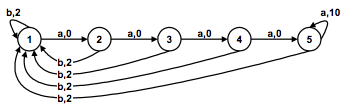
\includegraphics[width=0.4\textwidth]{chain.png}
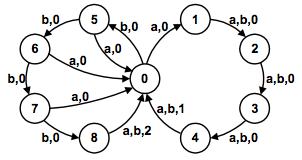
\includegraphics[width=0.4\textwidth]{loop.png}
\caption{\label{fig:chainloop} The ``Chain'' and ``Loop'' toy problems used in testing.}
\end{figure}

\begin{figure}
\centering
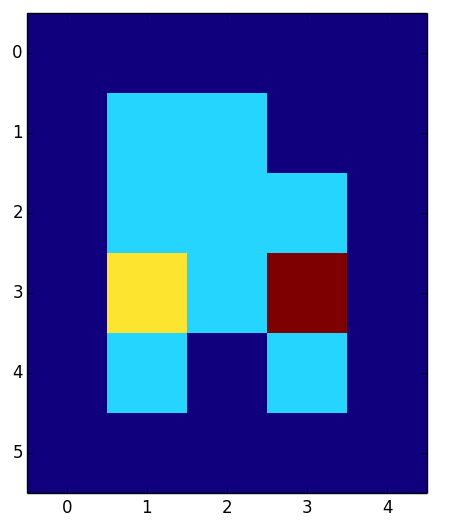
\includegraphics[width=0.2\textwidth]{easymaze.png}
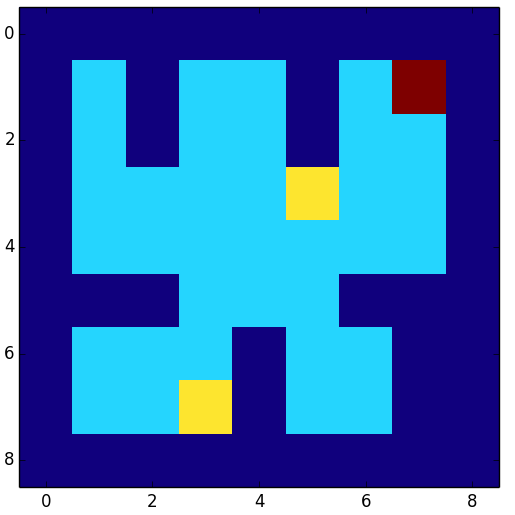
\includegraphics[width=0.25\textwidth]{hardmaze.png}
\caption{\label{fig:maze} The ``Maze'' flag-collecting toy problem used in testing.
Yellow squares are flags; red is the goal; all mazes start at the top left corner.}
\end{figure}

\subsection{Preliminary Results}
For the chain and loop problems, we performed learning phases of 5000 time steps. For
the easy maze problem, we performed learning phases of 2000 time steps, and for the hard
maze problem, we performed learning phases of 5000 time steps. In each of these
problems, there is a clear optimal policy and optimal reward. For the chain problem,
because the agent slips an average of 0.2 times, the optimal behavior on average receives
a total reward of approximately 20000 for 5000 steps. For the loop problem, the optimal
behavior receives a total reward of 2000 for 5000 steps. In the maze problem, the
probability of slipping makes it less clear what the optimal policy and total reward
would be in the end. We estimate that each slip adds an extra step in on the optimal
path, so the optimal reward for the easy maze is between 410 and 420 (with 2000 steps),
and between 540 and 550 for the hard maze (with 5000 steps).


\bibliographystyle{apalike}
\bibliography{writeup}

\end{document}
